\documentclass[__minimum__.tex]{subfiles}

\begin{document}

\paragraph{Дифракционный интеграл:}
$$
    E(P)
    =
    \frac{1}{i\lambda}\iint\limits_{\Sigma'} \widetilde K(\psi) E(Q)\frac{e^{ikR}}{R}d\sigma,
$$
где $\Sigma'$ - открытая часть поверхности $\Sigma$, $Q$ - точка на $\Sigma'$, $E(Q)\frac{e^{ikR}}{R}$ - сферическая волна, идущая от этой точки, $\widetilde K(\psi)-$ медленно и монотонно убывающая функция, достигающая своего максимума в $R_0$ \\
\paragraph{Принцип Гюйгенса - Френеля:}
\begin{enumerate}
    \item
          Если окружить систему когерентных источников произвольной замкнутой поверхностью $\Sigma$, то каждую точку этой поверхности можно считать источником вторичных когерентных сферических волн, распространяющихся по всем направлениям. Амплитуда этих волн на поверхности находится как суперпозиция волн, идущих от первичных источников. Световое поле в любой точке вне этой поверхности можно рассчитывать как суперпозицию всех вторичных волн.
    \item
          Если часть этой поверхности закрыта непрозрачным экраном, то учитывать нужно только волны, идущие от открытых частей поверхности.
\end{enumerate}
\paragraph{Метод зон Френеля:} суть наблюдаемого эффекта заключается в том, что при изменении в определенных пределах радиуса диафрагмы в точке $P$ наблюдается то светлое, то темное пятно. Для объяснения этого эффекта Френель предложил разбить вспомогательную поверхность на зоны. Первая зона Френеля представляет собой шапочку на сфере, граница которой отстоит от точки $P$ на расстояние $R_1 = R_0 + \frac{\lambda}{2}$, так что ей принадлежат все точки сферы в пределах $R_0 < R < R_0 + \frac{\lambda}{2}$. Все остальные зоны - пояса. Вторая зона задается условиями $R_0 + \frac{\lambda}{2} < R < R_0 + \frac{2\lambda}{2}$, ее внешняя граница удалена от точки наблюдения на расстояние $R_2 = R_0 + \frac{2\lambda}{2}$. Для $m$-той зоны:
$$
    R_{m-1} < R < R_m,
$$
$$
    R_m = R_{m-1} + \frac{\lambda}{2} = R_0 + m\frac{\lambda}{2}
$$
Используем формулу
$$
    E=E_0\left(K(R_{min}) e^{ik(R_{min} - R_0)} - K(R_{max})e^{ik(R_{max} - R_0)} \right)
$$
В случае, если диафрагма открывает первую зону Френеля:
\begin{gather*}
    R_{min} = R_0, \qquad R_{max} = R_0 + \frac{\lambda}{2} , \\
    e^{ik(R_{min} - R_0)} = 1, \qquad e^{ik(R_{max} - R_0)} = e^{ik\frac{\lambda}{2}} = e^{i\pi} = -1
\end{gather*}
Поле от первой зоны Френеля:
$$
    E^{(1)} = E_0(1 + K(R_1))
$$
Аналогичные расчеты дадут для второй зоны Френеля:
$$
    E^{(1)} = - E_0(K(R_1) + K(R_2))
$$
Для $m$ - той зоны:
\begin{gather*}
    R_{min} = R_0 + (m - 1)\frac{\lambda}{2}, \qquad R_{max} = R_0 + m\lambda \\
    e^{ik(R_{min} - R_0)} = e^{\frac{i(m-1)k\lambda}{2}} = e^{i(m-1)\pi} = (-1)^{m-1}, \qquad
    e^{ik(R_{max} - R_0)} = e^{ikm\frac{\lambda}{2}} = e^{im\pi} = (-1)^m\\
    E^{(m)} = E_0\left((-1)^{m-1} K(R_{m-1}) - (-1)^m K(R_m)\right) = E_0(-1)^{m-1} (K(R_{m-1}) + K(R_m))
\end{gather*}

\paragraph{Интенсивность:} скалярная физическая величина, количественно характеризующая мощность, переносимую волной в направлении распространения. Численно интенсивность равна усреднённой за период колебаний волны мощности излучения, проходящей через единичную площадку, расположенную перпендикулярно направлению распространения энергии. В математической форме это может быть выражено следующим образом:
\begin{gather*}
    I(t) = \frac{1}{T}\int_0^{t+T}\frac{dP}{dS}dt,
\end{gather*}
где $T$ - период волны, $dP$ — мощность, переносимая волной через площадку $dS$.
Интенсивность волны связана со средней плотностью энергии $W$ в волне и скоростью распространения волны $\nu$ следующим соотношением:
\begin{gather*}
    I = W\nu.
\end{gather*}
Единицей измерения интенсивности в Международной системе единиц (СИ) является Вт/м².
Электромагнитное излучение (например, свет) представляет собой совокупность волн, колебания в которых совершают напряжённость электрического поля и магнитная индукция. Электромагнитные волны переносят энергию электромагнитного поля, поток которой определяется величиной вектора Пойнтинга. Интенсивность электромагнитного излучения равна усреднённому за период значению модуля вектора Пойнтинга.
\begin{gather*}
    I(t)=\frac{1}{T}\int_0^{t+T}\big|\vec{S}(t)\big|dt,
\end{gather*}
где вектор Пойнтинга $\vec{S}(t) = \big[\vec{E}(t)\times\vec{B}(t)\big]$(в системе СГС) $E$ — напряжённость электрического поля, $B$ — магнитная индукция.

\paragraph{Условия интерференции:}
\begin{enumerate}
    \item
          Ортогональность поляризаций волн.
          При этом $\vec{E}_{10}\perp\vec{E}_{20}$. Интерференционные полосы отсутствуют, а контраст равен $0$. Далее, без потери общности, можно положить, что поляризации волн одинаковы.
    \item
          В случае равенства частот волн ${\mathbf  {}}\Delta \omega = 0$ и контраст полос не зависит от времени экспозиции $V=\frac{2\left<\vec{E}_{10},\vec{E}_{20}\right>}{I_1+I_2}$\\
    \item
          В случае ${\mathbf  {}}\Delta \omega \tau \gg 2\pi$   (радиан) значение функции   ${\displaystyle \mathrm {sin} ({\frac {\Delta \omega \tau }{2}})\simeq 0}$  и интерференционная картина не наблюдается. Контраст полос, как и в случае ортогональных поляризаций, равен $0$.
    \item
          В случае ${\mathbf  {}}\Delta \omega \tau <2\pi$   контраст полос существенным образом зависит от разности частот и времени экспозиции.
\end{enumerate}
Интенсивность излучения при интерференции:
\begin{gather}
    \label{o-02-mainint}
    I = I_1 + I_2 + 2\sqrt{I_1 I_2}\langle\cos(\Delta \varphi)\rangle
\end{gather}
где $2\sqrt{I_1 I_2}\langle\cos(\Delta \varphi)\rangle$ называется интерференционным членом.

\begin{wrapfigure}{R}{0.4\linewidth}
    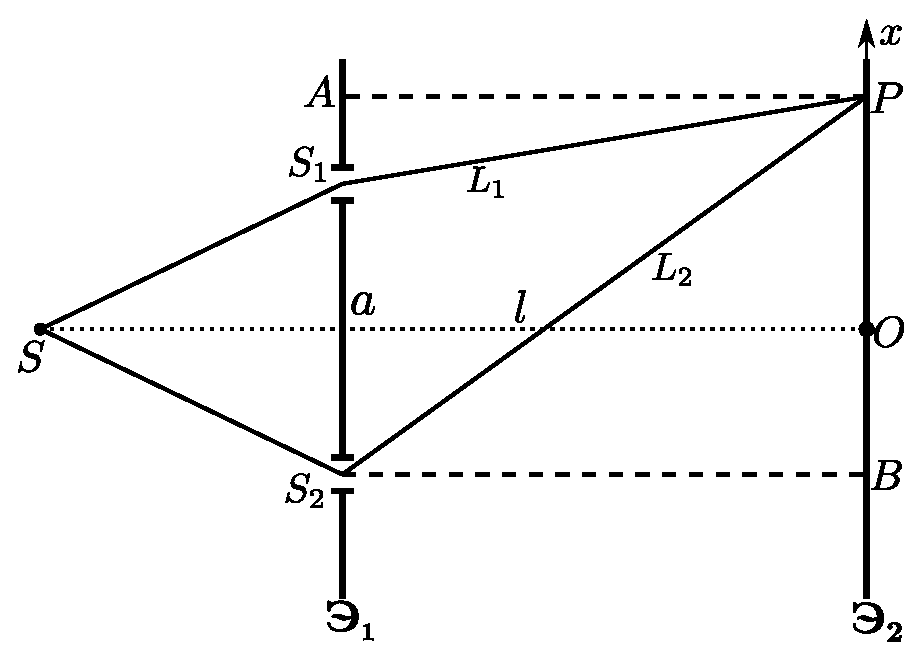
\includegraphics[width=1\linewidth]{img/o-02}
    \caption{Общая схема наблюдения интерференции}
    \label{o-02-scheme}
\end{wrapfigure}

\textbf{Схема наблюдения интерференции:} световые лучи от источника $S$ проходят через две щели на экране $\text{Э}_1$, образуя два источника $S_1$ и $S_2$. Лучи от этих источников попадают на экран $\text{Э}_2$, на котором наблюдается интерференционная картина в виде плавно переходящих друг в друга светлых полос, перпендикулярных плоскости рисунка.

Отыщем вид (\ref{o-02-mainint}) для этой схемы, для этого найдем $\Delta = L_2 - L_1$. Из
$\triangle S_1AP$ и $\triangle S_2BP$ отыщем $L_1$ и $L_2$ (см. Рис. \ref{o-02-scheme}):
$$
    L_1 = \sqrt{l^2 + \left(x-\frac{a}{2}\right)^2}, \qquad
    L_2 = \sqrt{l^2 + \left(x+\frac{a}{2}\right)^2},
$$
положим $l \gg a, \ l \gg |x|$ и воспользуемся теоремой Тейлора для $L_1$ и $L_2$:
\begin{gather*}
    L_1 \approx l + \frac{\left(x-a/2\right)^2}{2l}, \qquad
    L_2 \approx l + \frac{\left(x+a/2\right)^2}{2l},
\end{gather*}
тогда
\begin{gather}
    \label{o-02-schemediff}
    \displaystyle \Delta = L_2 - L_1 = \frac{xa}{l}
\end{gather}
Запишем формулу для интенсивности (\ref{o-02-mainint}) с учетом (\ref{o-02-schemediff}):
\begin{gather*}
    I = I_1 + I_2 + 2\sqrt{I_1 I_2}\cos\left(\frac{2\pi}{\lambda}\Delta\right) =
    I_1 + I_2 + 2\sqrt{I_1 I_2}\cos\left(\frac{\pi x a}{\lambda l}\right),
\end{gather*}
для $I_1 = I_2 = I_0$:
\begin{gather}
    \label{o-02-intensesch}
    I = 2I_0\left(1 + \cos\left(\frac{2\pi}{\lambda}\Delta\right)\right) =
    4I_0\cos^2\left(\frac{\pi xa}{\lambda l}\right),
\end{gather}

\end{document}